\section{System Design and Implementation}
\label{sec:impl}

To test our hypothesis introduced \vpageref{hyp:anxiety}, we wanted to compare the following scenarios
\begin{inlinelist}
	\item \textit{climb in \gls{VR},} moving by using hand and footholds (\ref{cd:B})
	\item \textit{climb in \gls{VR},} by only using game controllers, like in the \gls{VR} game \href{https://en.wikipedia.org/wiki/The_Climb_(video_game)}{\textit{The Climb}, \citeyear{ClimbOfficialSite2016}} (\ref{cd:C}).
\end{inlinelist} In both cases, a participant would virtually be in a height of at least \SI{5}{\meter} (for comparability with \textcite{Pijpers2006}) but physically close to the floor. As ground truth---no pun intended---we introduced a third scenario (\ref{cd:A}): the participant performs real climbing at the same elevation as in the \gls{VE}, without any \gls{VR} equipment. \pdfmargincomment[avatar=peter,style=korrektur-done]{überarbeitet}

These scenarios induce various requirements we needed to find solutions for
\begin{inlinelist}
	\item a location to let the participants climb safely at two elevations low and high
	\item a \gls{VE} reproducing the visual impression of climbing under the high condition with two different levels of interaction
	\item a way of metering psychosomatic anxiety
	\item means of measuring presence. 
\end{inlinelist} Throughout the following subsections, we describe how we met these requirements.

\subsection{Climbing Routes}

We were allowed to conduct our experiment in \href{https://www.kletterzentrum-bremen.com/}{a climbing gym located nearby the campus}, with a wall that fulfills the specifications for one lane of an \gls{IFSC} speed climbing wall. We chose this wall (Figure \ref{fig:climbing-wall-photo}) to host our traversal routes for two reasons
\begin{inlinelist}
	\item it is angled at a constant \SI{5}{\degree} along its entire length
	\item it is easily accessible on the ground floor and from a balcony at about \SI{10}{\meter}.
\end{inlinelist}
By letting our participants climb the same horizontal route (Figure \ref{fig:climbing-wall-schema}) at a constant elevation in each condition, we maintained comparability with \textcite{Pijpers2003} and kept height---our main trigger for anxiety---at a constant level. \pdfmargincomment[avatar=peter,style=korrektur-done]{überarbeitet}

\begin{figure}[ht]
	\centering
	\begin{subfigure}[t]{.4825\textwidth}
		\vspace*{\fill}
		\centering
		\includegraphics[width=\textwidth]{include/images/climbing-wall-photo.jpg}
		\subcaption{Total view of the \gls{IFSC} lane}
		\label{fig:climbing-wall-photo}
	\end{subfigure}%
	\hfill
	\begin{subfigure}[t]{.48\textwidth}
		\vspace*{\fill}
		\centering
		\hspace*{-0.8cm}
		\includegraphics[width=\textwidth]{include/images/climbing-wall-schema.pdf}
		\subcaption{Schematic view of the traversal routes}
		\label{fig:climbing-wall-schema}
		\par\vspace*{0.25cm}
		\includegraphics[width=\textwidth]{include/images/hold-photo.jpg}
		\subcaption{Hand holds (w: \SI{12}{\cm}, h: \SI{4/6}{\cm}, d: \SI{4}{\cm})}
		\label{fig:hold-photo}
	\end{subfigure}
	\captionsetup{subrefformat=parens}
	\caption[Climbing routes]{Two identical traversal routes at different heights \subref{fig:climbing-wall-schema}, each consisting of 14 hand and footholds made from wood \subref{fig:hold-photo}; T\textsubscript{h/f} mark the holds at the turning point}
	\label{fig:holds}
\end{figure}

A carpenter manufactured the holds from wood (Figure \ref{fig:hold-photo}), so they could easily be interspersed with the existing routes to keep unduly obstructions of the commercial operations at a minimum. Figure \vref{fig:climbing-wall-schema} shows the final route layout for condition \ref{cd:A} (\SI{10}{\meter}) and its twin at the bottom of the wall for condition \ref{cd:B} and \ref{cd:C}. Both routes have a launching platform made of plywood, each serving as the start and end point for the climbing task. Several experienced testers estimated the route's \glsdisp{UIAA}{UIAA} climb degree at 4+ so that even beginners could complete it. \pdfmargincomment[avatar=peter,style=korrektur-done]{überarbeitet}


\subsection{Virtual Reality}

We used the aforementioned climbing gym as a reference for the \gls{VR} scene and started modeling it, using an already existing architectural 3D model as a foundation. We continued by adding textures and lighting as well as some interior such as tables and fire extinguishers. By resembling the original premises with such details as furniture, we created points of reference in support of a sense for scale and height.

The climbing routes, sketched in Figure \vref{fig:holds}, required for the \gls{VR} conditions \ref{cd:B} and \ref{cd:C} were added too. To reduce the risk of injuries by unexpected collisions with other holds that are not part of the traversal, we added a photogrammetric scan of the wall at first. Unfortunately, right before the experiments begun, the commercial routes were changed, and we had to remove the scan.

We utilized \href{https://www.autodesk.com/products/maya/overview}{Autodesk Maya} for modeling and \href{https://unity3d.com/}{Unity 3D} as a game engine to create an interactive experience. Further, we used an \href{https://www.vive.com/}{HTC VIVE} system for tracking the head, two controllers, and two additional trackers for the feet. Lastly, for tracking the hands, we employed a \href{https://www.leapmotion.com/}{Leap Motion} hand tracking device mounted on the VIVE headset using a 3D-printed version of its official \href{https://store-us.leapmotion.com/products/universal-vr-mount-pre-order}{universal mount}, see Figure \ref{fig:leap-motion-setup}.

\marginpar{%
	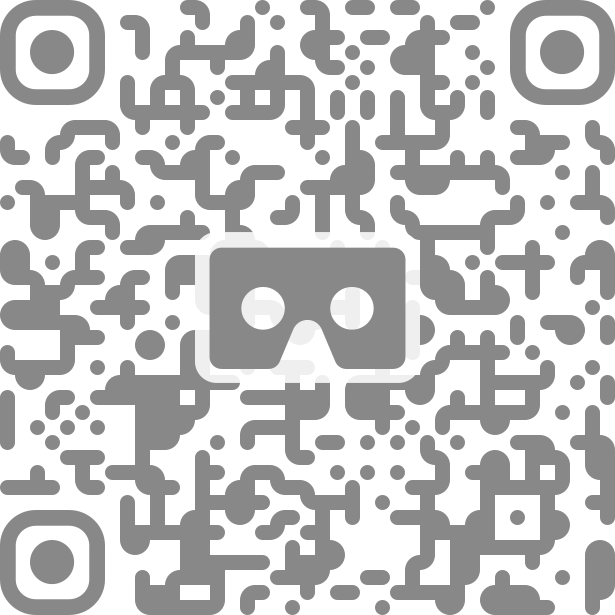
\includegraphics[width=\marginparwidth]{./include/images/qr-code.pdf}
	\captionsetup[figure]{font={sf,stretch=1.0}}
	\captionof*{figure}{%
		\textcolor{gray}{%
			\href{https://www.youtube.com/watch?v=pFF6uI3PrZQ&fs=1&loop=1}{Have a look at the VR scene as interactive 3D video \faicon{youtube-play}}}}
}

To use a VIVE system it has to be set up first. That involves placing the base stations, called lighthouses, and calibrating the play space. Once that procedure has been completed successfully, the VIVE system calculates the 6D poses of all tracked devices within the reference frame of that play area. As not to break the immersion, we hid the chaperon marking out that area.

\subsubsection*{Robust Tracking}

The recommended position of the lighthouses is facing each other at a distance of \SI{5}{\meter} as well as above head height and angled down by \SIrange{30}{45}{\degree} \autocite{HTCVIVEDeveloper2018}. Preliminary tests revealed, though, that these recommendations do not work for tracking climbers on a wall due to issues with shading.

\begin{figure}[ht]
    \centering
    \begin{subfigure}[t]{0.289\textwidth}
        \centering
        \includegraphics[width=\textwidth]{include/images/vive-setup-problem.jpg}
        \caption{Climber with headset}
        \label{fig:vive-setup-problem}
    \end{subfigure}
    \hfill
    \begin{subfigure}[t]{0.699\textwidth}  
        \centering 
        \includegraphics[width=\textwidth]{include/images/vive-setup-solution.jpg}
        \caption{Placement of VIVE lighthouses}
        \label{fig:vive-setup-solution}
    \end{subfigure}
	\captionsetup{subrefformat=parens}
    \caption[VIVE setup]{Modified VIVE setup \subref{fig:vive-setup-solution} for optimal coverage of climbers on a wall even if they are in a typical pose \subref{fig:vive-setup-problem} where their arms cover up the headset}
    \label{fig:vive-setup}
\end{figure}

Figure \ref{fig:vive-setup-problem} shows a climber in a typical pose, hanging on his stretched out arms looking down towards his feet. This way, however, the VIVE headset is shaded from the lighthouses' infrared flashes, which have to hit the headset so the VIVE system can calculate its pose. To overcome this problem, one of the lighthouse base stations was placed \SI{50}{\cm} above the ground, angled up by \SI{45}{\degree} (Figure \ref{fig:vive-setup-solution}).

\subsubsection*{Registration---A Perfect Match}

For condition \ref{cd:B}, we needed static passive haptics. These have to be aligned with their representations in the \gls{VE}, so they can be interacted with. Since a permanent setup was not possible at the climbing gym, the so called registration process would have to be performed preceding every experiment session. To achieve the best possible registration nonetheless this procedure was at least semi-automated by creating a Unity component performing the alignment based on two VIVE trackers.

A general solution for such point cloud registration in 3D space requires at least three points. However, in this particular scenario some restrictions apply \begin{inlinelist}
\item{the only possible rotation axis is Y (up) since the tracked space (inside the actual climbing gym) and the virtual model (of that climbing gym) are placed on a flat, level floor}
\item{there is only translation and rotation involved (no scaling) since the \gls{VR} system already respects the scale of the Unity world}
\end{inlinelist}. Therefore, aligning the tracker positions with their predefined counterparts inside Unity essentially becomes a 2D problem that can be solved as follows: First, translate the reference frame of the trackers (the camera rig) so the centroid of tracker positions and the counterpart positions correspond. Then rotate the rig around the Y-axis of that centroid, so each tracker gets as close to its counterpart as possible. We implemented this algorithm based on \textcite{Ho2013}.

\begin{figure}[ht]
	\centering
	\begin{subfigure}[t]{0.49\columnwidth}
		\centering
		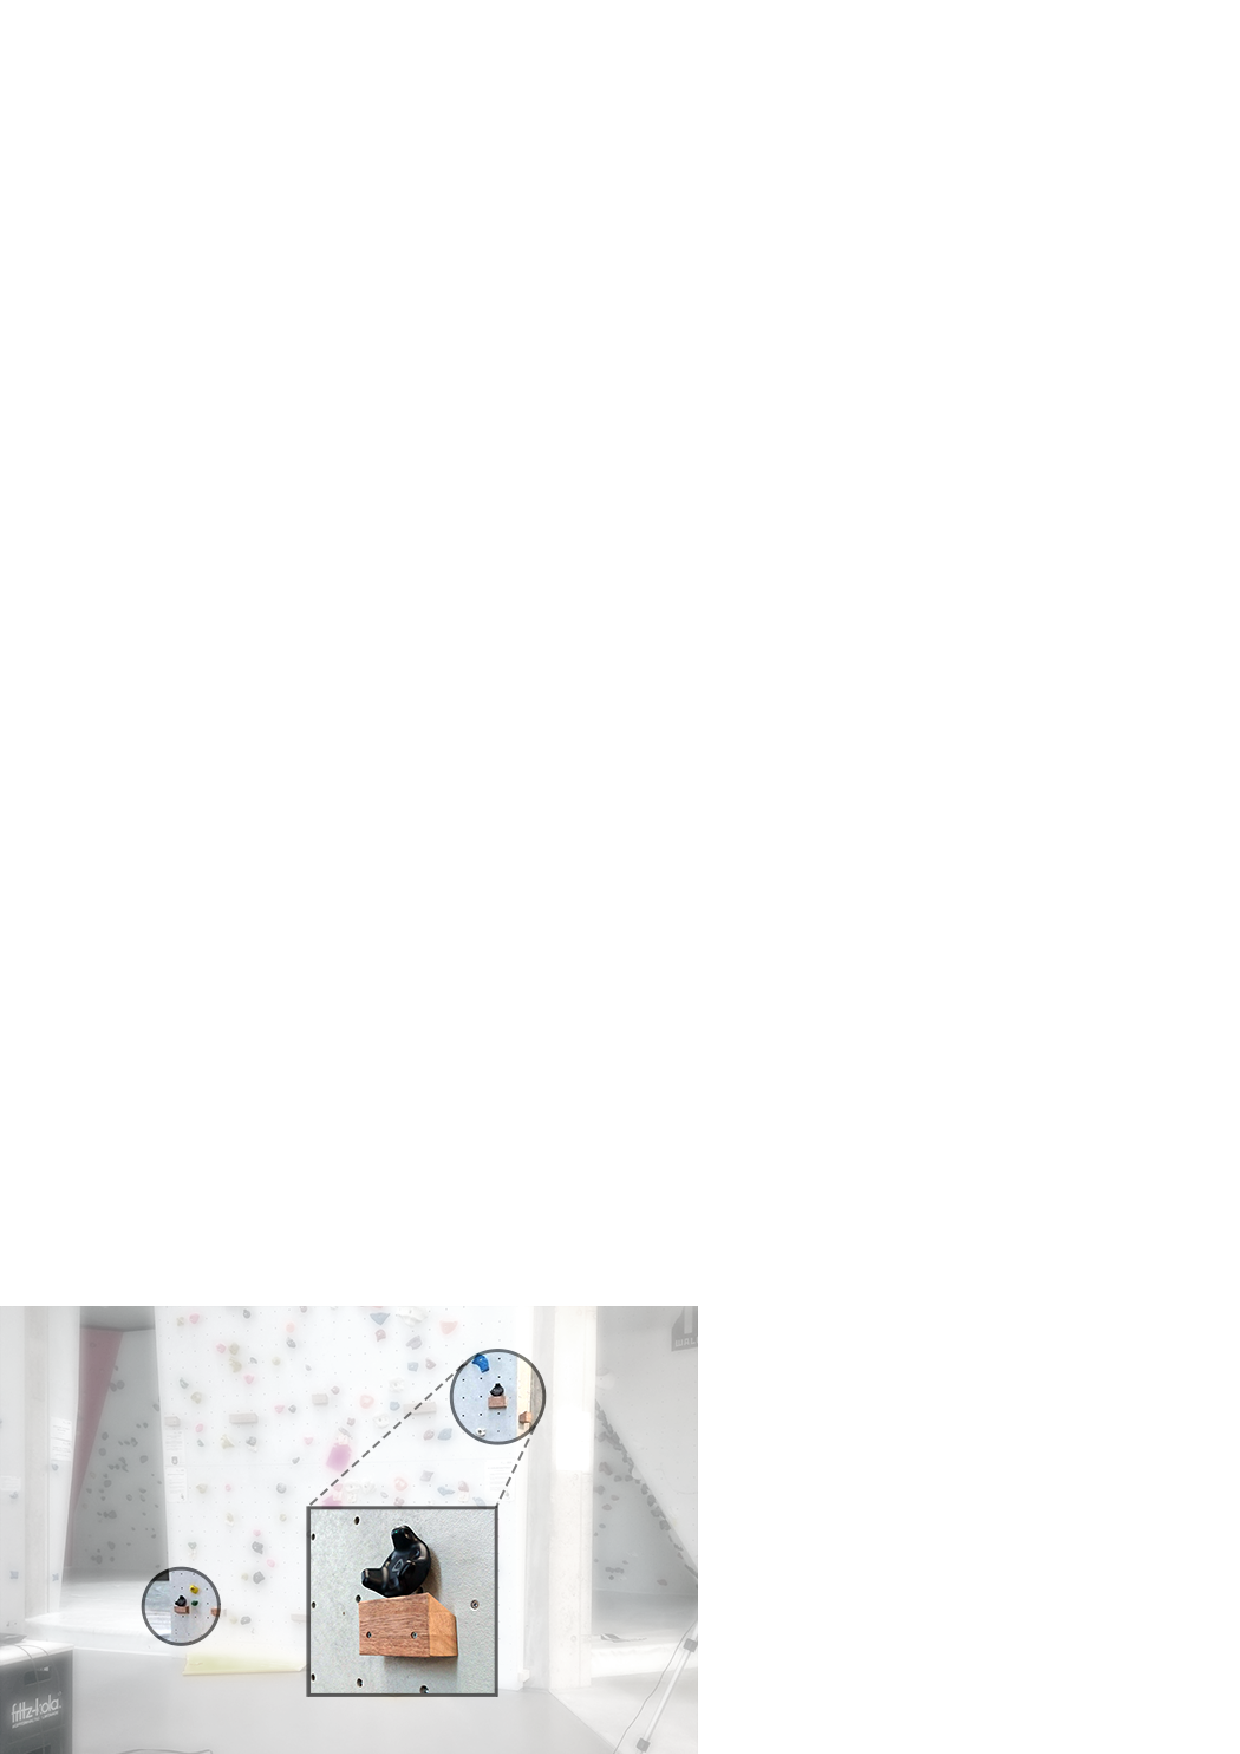
\includegraphics[width=\textwidth]{include/images/registration-trackers.png}
		\caption{Placement of the VIVE trackers in the traversal on top of a hand- and foothold (in circles)}
		\label{fig:registration-trackers}
	\end{subfigure}
	\hspace*{\fill}
	\begin{subfigure}[t]{0.49\columnwidth}
		\centering
		\includegraphics[width=\textwidth]{include/images/registration-unity.png}
		\caption{Screenshot of the registration component in Unity which performs the alignment of tag object pairs, for example, “left tracker”}
		\label{fig:registration-unity}
	\end{subfigure}
	\caption[VIVE play area registration]{Semi-automated registration of the VIVE play area with the real world}
	\label{fig:registration}
\end{figure}

Whenever the VIVE system was set up, two of its trackers where placed in the climbing route, see Figure \ref{fig:registration-trackers}, and the registration component was used to calculate a transform to align them with their corresponding positions on the virtual climbing wall, see Figure \ref{fig:registration-unity}. For inscrutable reasons, the orientation of the play area occasionally changed during the experiment sessions and required a renewed registration.

\subsubsection*{Climbing}

For condition \ref{cd:B} participants are physically climbing, by moving through the room using passive props as hand and footholds. Therefore, they need representations of hands and feet that we realized as follows.

\paragraph{Hands} We wanted to provide the participants with a hand representation as close to their own hands as possible; therefore, we chose an image-based approach. The Leap Motion system used for that purpose provides two things: Stereo infrared images and poses of tracked hand and finger joints, provided that hands could be extracted from the images \autocite{Colgan2014}. Leap Motion provides generic, rigged hand models ready to be used, yet, pretests showed that they are not an option for two reasons: First, the proportions of hand model and original hand do not match, which causes a discrepancy between what can be seen and what can be felt, for example, when touching one hand with the other. Second, the Leap Motion system cannot extract hands when they cling to hand holds. To work around this issue, we came up with an alternative hand representation inspired by \textcite{Colgan2015}. 

For our setup, we implemented hand visuals as a masked, tinted overlay of the infrared image coming from the Leap Motion camera. To create that in Unity the raw infrared image is initially projected onto a camera-spaced canvas using a custom shader. For the mask, a second off-screen camera renders a single layer containing only the generic hand models with the captured joint poses and stores it in a texture. Additionally, we gave the hand meshes a white, light-emitting material and enabled a blurring post-processing-filter to achieve smooth edges of the mask. The final masked overlay can be seen in Figure \ref{fig:leap-motion-overlay-result}.

As indicated earlier, the Leap Motion system cannot capture hands outside the sensor's field of view. Although the system is capable of guessing the pose of joints that \textit{become} hidden from the camera, it cannot extract hands \textit{already} partially hidden when they enter the field of view. By default, Leap Motion's Unity integration hides models of lost hands, but in our case, that yields an utterly translucent mask and, therefore, a fully transparent overlay. To work around this, we tweaked the default behavior, such that models are no longer hidden. Instead, they are frozen in the last valid tracked pose before they leave the field of view. Until tracking is re-established the masking hand model hence remains at the same frozen position in space. Even if Leap Motion cannot extract a hand, its infrared image is still visible through the old mask as long as that hand is not moved too far away.

\begin{figure}[ht]
    \centering
        \begin{subfigure}[t]{0.32\textwidth}
    	\centering
       	\includegraphics[width=\textwidth]{include/images/leap-motion-overlay-setup.jpg}
    	\caption{The Leap Motion sensor mounted on VIVE headset}
    	\label{fig:leap-motion-setup}
    \end{subfigure}
    \hfill
    \begin{subfigure}[t]{0.32\textwidth}
        \centering
       	\includegraphics[width=\textwidth]{include/images/leap-motion-overlay-photo.jpg}
        \caption{Photo of a right hand over a handhold}
        \label{fig:leap-motion-overlay-photo}
    \end{subfigure}
    \hfill
	\begin{subfigure}[t]{0.32\textwidth}
		\centering
		\includegraphics[width=\textwidth]{include/images/leap-motion-overlay-result.jpg}
		\caption{Screenshot of the resulting, masked infrared overlay}
		\label{fig:leap-motion-overlay-result}
	\end{subfigure}
	\captionsetup{subrefformat=parens}
    \caption[Leap Motion hand tracking]{Leap Motion hand overlay created from the infrared image provided by the sensor \subref{fig:leap-motion-setup} masked with a blurred image of the rendered hand models, which makes objects near the hands, such as the hand holds, visible as well \subref{fig:leap-motion-overlay-result}}
    \label{fig:leap-motion-overlay}
\end{figure} 

\paragraph{Feet} Footwork and technique are essential in climbing \autocites{Sheldon2014}[based on][]{Anderson2014}. Therefore, besides capturing the hands, a precise foot tracking was implemented using VIVE trackers. While climbing, the feet are pointed towards the wall most of the time, and, since they are also close to the wall, the chance of them being hidden from the VIVE base stations is increased. To work around that, the trackers were attached to the heel instead of the instep, using a tripod screw, which itself is drilled through the rear rubber band of a grounding heel strap, and padded with a scouring pad, as shown in Figure \ref{fig:foot-tracking-tracker}. As a result, the tracking rarely gets lost and allows precise foot placement.

\begin{figure}[ht]
    \centering
    \begin{subfigure}[t]{0.49\textwidth}
        \centering
		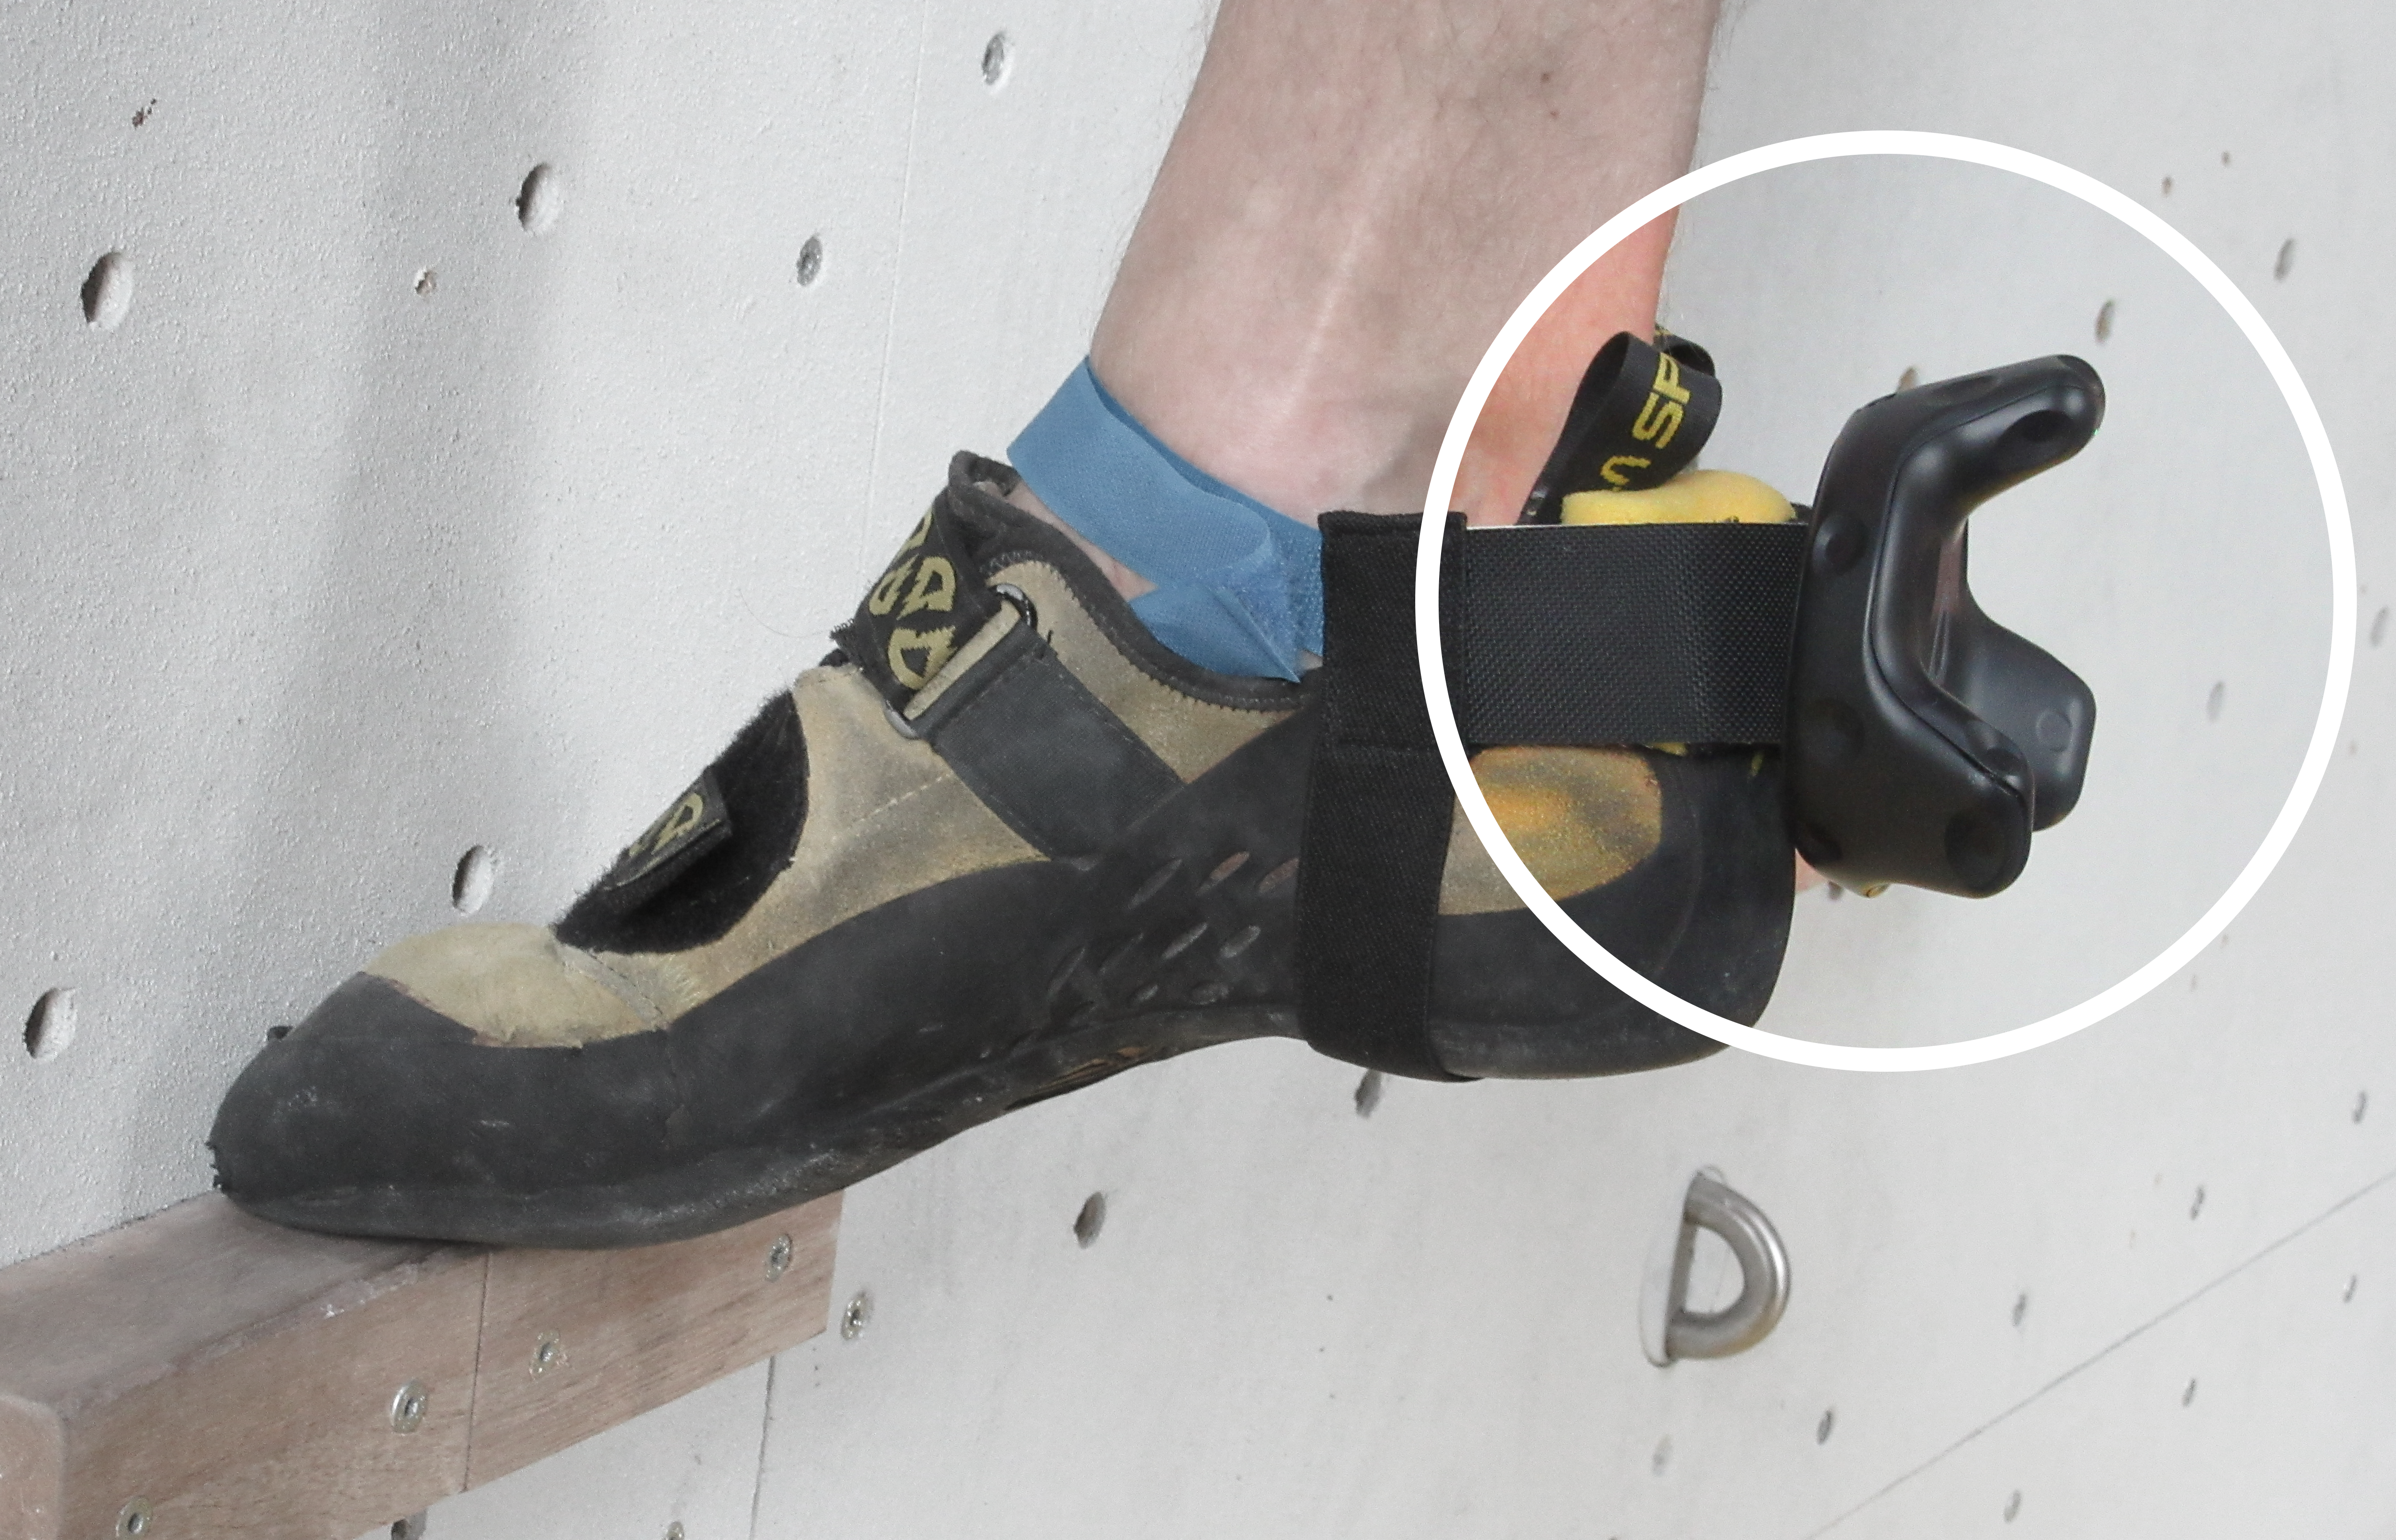
\includegraphics[width=\textwidth]{include/images/foot-tracking-tracker.png}
		\caption{Heel-mounted VIVE tracker (circled)}
        \label{fig:foot-tracking-tracker}
    \end{subfigure}
    \hfill
    \begin{subfigure}[t]{0.49\textwidth}  
        \centering 
		\includegraphics[width=\textwidth]{include/images/foot-tracking-result.png}
		\caption{Captured climbing shoe model in Unity}
        \label{fig:foot-tracking-result}
    \end{subfigure}
    \caption[VIVE foot tracking]{Foot tracking with heel-mounted VIVE trackers which are attached using a pair of modified grounding heel straps}
    \label{fig:foot-tracking}
\end{figure}

Looking back from the experiment sessions, we encountered two issues: First, because of the materials (rubber bands, sponge) used for the mount, it is sensitive to shocks, for example, when---due to limited space on a foothold---the heels collide. Second, due to the position of the tracker over the heel, a small offset in its default position substantially shifted the tip of the foot. That made it hard to calibrate the feet reproducibly and lead to the tips occasionally being off by centimeters. An alternative mount on top of the instep as done by \textcite{Tiator2018} might yield more stable results.

\subsection{Questionnaire Software}

To reduce overhead and eliminate transfer errors, the survey software \href{https://www.limesurvey.org/}{LimeSurvey 3.7.0}\footnote{\url{https://www.limesurvey.org/}} was employed to collect answers to the questionnaires used throughout the study. To do so, we had to implement the following extensions\begin{inlinelist}
	\item visual analog scales (anxiety thermometer and \gls{RPE})
	\item question group order per participant achieve the randomized order of conditions
\end{inlinelist}.

\subsection{Physiological Measures}

Besides self-evaluation, stress exertion and stress were to be metered through physiological measures, too, namely \glsfirst{HR}, \glsfirst{RR}, and \glsfirst{EDA}. We recorded them with a BITalino (r)evolution Plugged Kit BT, a \href{http://bitalino.com/en/plugged-kit-bt}{“versatile and scalable hardware platform for biosignals acquisition and wireless transmission in real-time.”} \autocite{BITalinoBoardKit}. This system acquires signals from up to six analog channels at a rate of up to \SI{1}{\kilo\hertz} and transmits them to a receiver via Bluetooth. We utilized \href{https://store.plux.info/electrodes/60-non-gelled-reusable-agagcl-electrodes.html}{non-gelled reusable Ag/AgCl electrodes} coated with \href{https://store.plux.info/electrodes/70-ten20-conductive-paste-for-eeg-810122129.html}{Ten20 conductive paste} for \gls{ECG} and \gls{EDA} signal acquisition, which we fixated on the skin using non-woven adhesive dressing.

For the placement of the electrodes we had to compromise between optimal signal strength and practicability. Since we wanted to derive \gls{HRV} from the \gls{ECG} signal, we chose to place the electrodes for rhythm monitoring \autocite{ECGLeadPlacement2015}. For a three-electrode setup, the upper electrodes are usually placed near the outer end of the collarbone \autocite{Klabunde2017,EKGPlatzierung2007}. To reduce motion artifacts---due to the expectable movement while climbing---we placed the upper electrodes \textit{above} the collar bone, closer to the neck, see Figure \ref{fig:electrodes-schema}, which still gave usable results. Also, a regular heart rate monitor, the \href{https://de-eu.wahoofitness.com/devices/heart-rate-monitors/wahoo-tickr-x-heart-rate-strap}{wahoo TICKR X chest strap}, was used to provide an independent signal for checking the validity of the \gls{ECG} measurements.

\Gls{SCR} is commonly measured by \gls{EDA} electrodes placed at index and middle finger. Such placement is impractical when climbing, however, since the participants need their fingers to grab either the hand holds or the controllers. The same applies to a fitting on the feet, as suggested by \textcite{Bertle2014}. As an alternative, \textcite{vanDooren2012} suggest fixing the electrodes either at the forehead or at the shoulder, which still yield signals correlated to those measured between the fingers \autocite{vanDooren2012}. When placed at the forehead, the electrodes would have become prone to accidental displacement when putting on or taking off the \gls{VR} headset, and therefore the shoulder was chosen as the only practical placement option, see Figure \ref{fig:electrodes-schema}.

\begin{figure}[ht]
    \centering
    \begin{subfigure}[t]{0.49\textwidth}
        \centering
		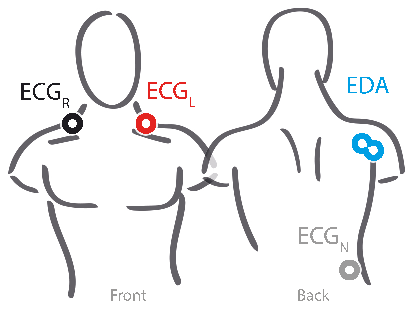
\includegraphics[width=\textwidth]{include/images/electrodes.png}
		\caption{Schematic view of a torso with the placements of the \gls{ECG} and \gls{EDA} electrodes}
        \label{fig:electrodes-schema}
    \end{subfigure}
    \hfill
    \begin{subfigure}[t]{0.49\textwidth}  
        \centering 
		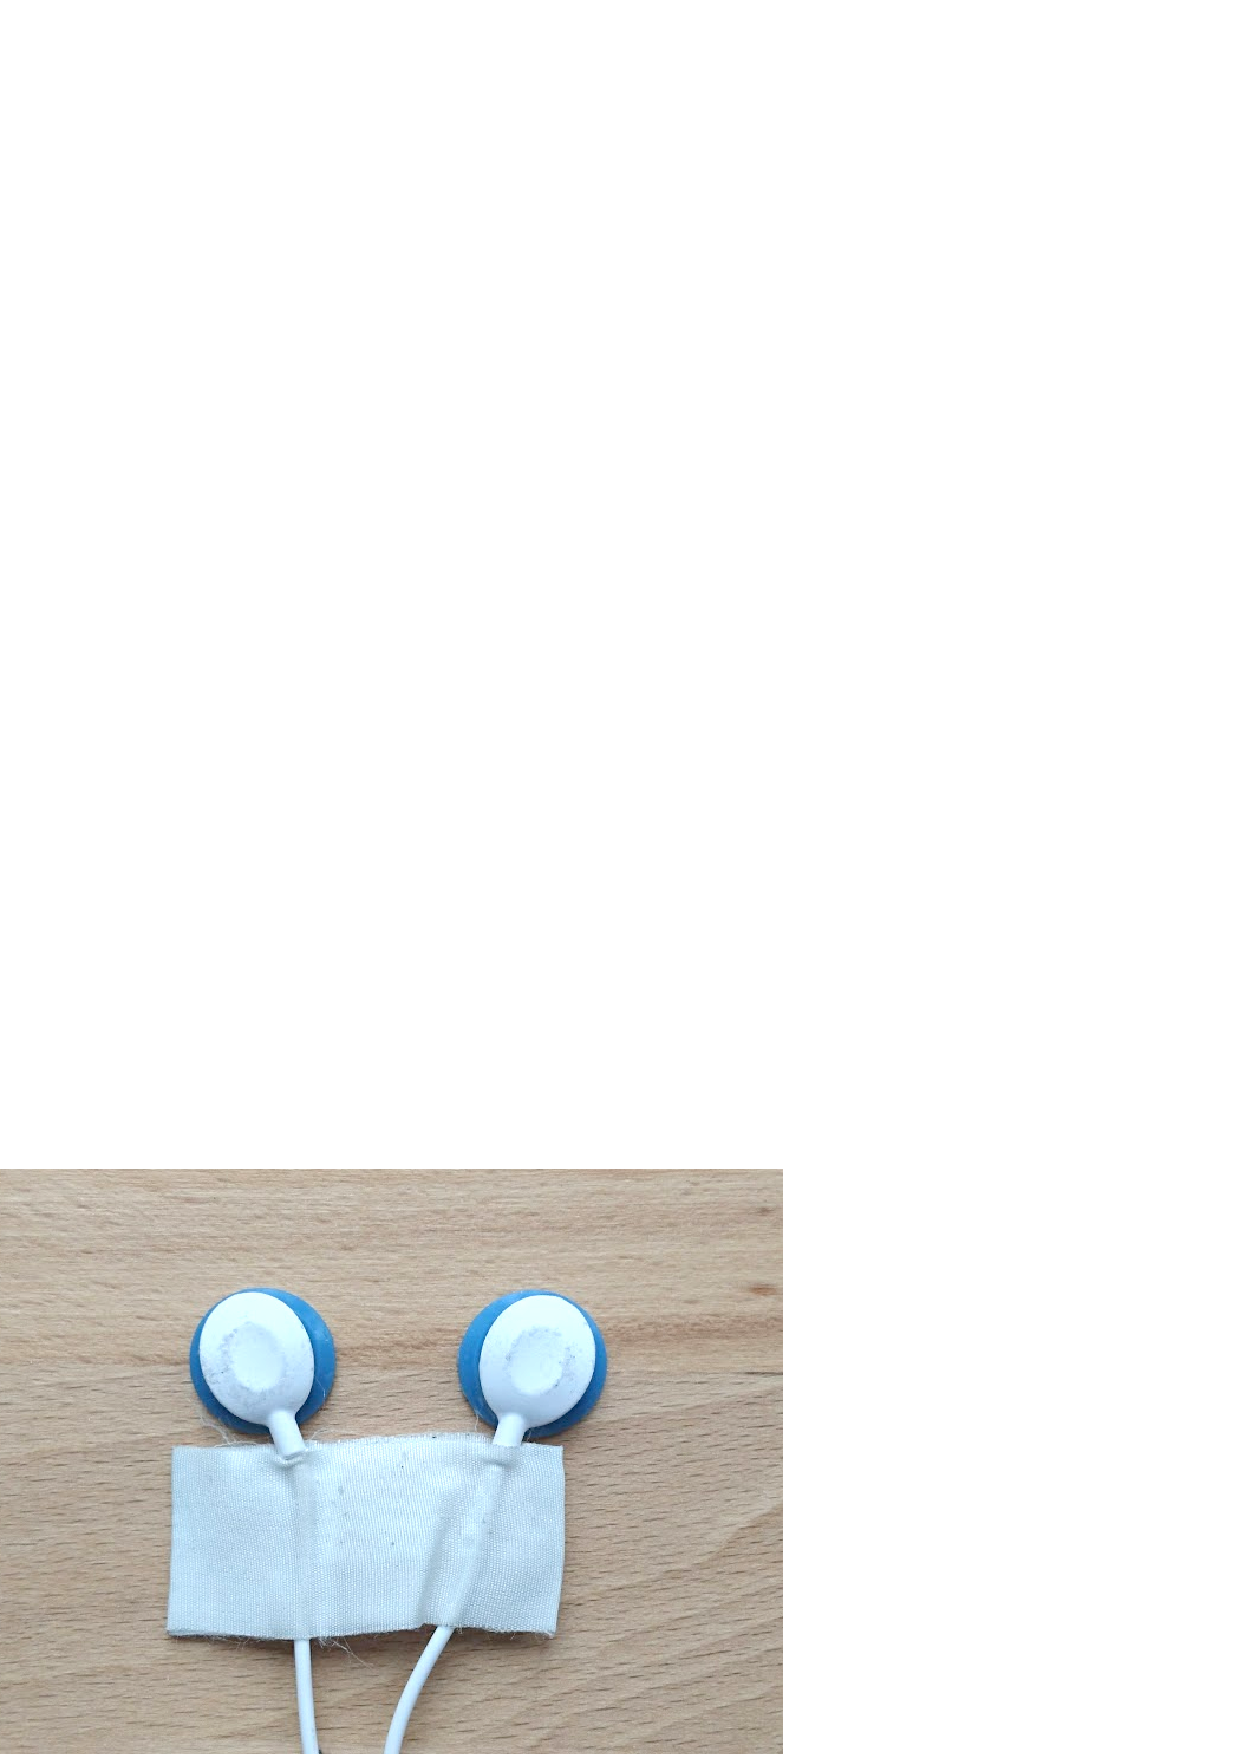
\includegraphics[width=\textwidth]{include/images/electrodes-eda.pdf}
		\caption{\gls{EDA} electrodes prepped with a piece of tape to keep them at a constant distance of \SI{5}{\centi\meter}}
        \label{fig:electrodes-eda}
    \end{subfigure}
    \caption[Placement of electrodes]{Electrodes for \glsfirst{ECG} and \glsfirst{EDA}}
    \label{fig:electrodes}
\end{figure}

BITalino provides a platform-independent (including Android and iOS) software called \href{http://bitalino.com/en/software}{OpenSignals (r)evolution} which provides real-time visualization and recording capabilities. Neither does this software allow tagging events and/or sections in a recording nor fusing the acquired signals with others such as video. However, a video recording in sync with biosignal recording was considered helpful for subsequent examination of potential outlier signals. Stress was expected to change throughout each condition, so we divided them into four following parts: preparation, way in, rest, and way out. Consequently, tagging these became a required feature as well.

\subsubsection*{Signal Recording with a Custom Android App}

Since we could not find an available software already fulfilling the required features, we developed a custom Android app tailored to our needs. Figure \ref{fig:android-app} shows the recorder screen providing all the required functionality: video and biosignal recording as well as tagging the parts of a condition mentioned above.

\begin{figure}[ht]
   \centering
   {
   	\includegraphics[width=0.49\textwidth]{include/images/android-app-photo.jpg}
   	\phantomsubcaption\label{fig:android-app-preview}
   	\phantomsubcaption\label{fig:android-app-parts}
   	\phantomsubcaption\label{fig:android-app-devices}
   }
   \captionsetup{subrefformat=parens}
   \caption[Android recorder]{Photo of the Android app recorder screen for recording video and biosignals from a BITalino and a Wahoo TICKR X, with a video preview \subref{fig:android-app-preview}, a list of connected devices, with their current state \subref{fig:android-app-devices}, as well as the buttons for tagging parts of the recording \subref{fig:android-app-parts}}
   \label{fig:android-app}
\end{figure}

Both devices used for signal acquisition, BITalino and wahoo TICKR X, support \gls{BLE} network technology for transferring data from the device to the phone running the recorder app. Both manufacturers offer Android support through a programming library, which encapsulates the low-level \gls{BLE} bonding process and the mapping of data fragments to Java objects. Implementation was done in Kotlin using Reactive Streams to channel all the sources of input (biosignal devices data and state changes, app state changes, and user input) and process the events in a non-blocking fashion.

Occasionally---the circumstances are still unknown---the BITalino device sent incomplete data; it responded frames with all six analog channels at the requested rate of \SI{100}{\hertz}, yet only every \engordnumber{100} frame contained valid values, all other frames were simply filled with nils. So we implemented a detector for this behavior which makes the user aware of the problem so the recording can be restarted.

\subsubsection*{Signal Postprocessing with Python}

The raw data acquired from the BITalino needs processing to extract features such as \gls{HRV}, or \gls{SCR}. This processing was done in python mainly using PANDAS (Data Analysis), and BioSPPy (Bio Signal Processing). BioSSPy is specialized in feature extraction, among other things, from \gls{ECG}, and \gls{EDA}, and \gls{RR} signals. Based on the processed output, further derived measures were calculated, like the \gls{HR} averaged over two respiration cycles as suggested by \autocite{Meehan2001}.

After processing the signals of participant, they were merged with their answers to the questionnaires stored on the LimeSurvey server. Some of these answers required postprocessing, for instance, mapping the degree at which they climb to one of three experience levels: beginner, average, and advanced.